\section{Prototipo di UI}
\label{ui}
Al fine di ottenere il prima possibile un feedback con il proponente riguardo all'interfaccia grafica del prodotto da sviluppare, è stato creato un prototipo di UI\glossario{}.

\subsection{Welcome Page}
La pagina iniziale del prodotto contiene una lista delle operazioni che l'utente può eseguire. Essa è pensata in modo tale da semplificare l'utilizzo dell'utente al primo lancio del programma e in contemporanea fornire all'utente esperto l'accesso alle funzionalità principali. A sinistra sono presenti dei pulsanti che consentono la \textit{creazione} e la \textit{modifica/visualizzazione} di elementi. Nella parte destra invece, sono presenti due pulsanti per l'avvio dell'analisi e la visualizzazione dei risultati delle precedenti analisi.
Inoltre, in ogni pagina, è presente un pulsante \textbf{Help}, che rimanda alla guida per l'uso del prodotto.
\begin{figure}[!h]
	\centering
	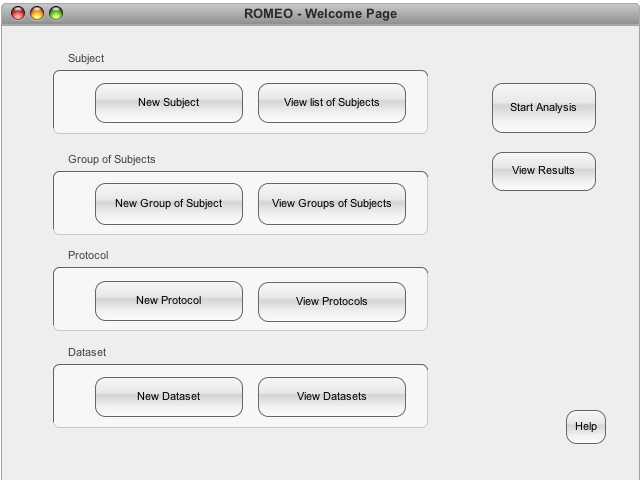
\includegraphics[width=0.8\linewidth]{./Content/Immagini/Prototype-v0.1/filesystemdoc_8_1}
	\caption{Romeo: Mock-up della pagina di benvenuto}
	\label{welcome_pages}
\end{figure}
\pagebreak
\subsection{Pagine di creazione}

\subsubsection{Creazione di un nuovo Subject}
In questa pagina sarà possibile inserire un nuovo subject\glossario{}, specificandone il \textit{nome}, caricando il file dell'immagine o del video e aggiungendo un eventuale maschera\glossario{}.
\begin{figure}[htp]
	\centering
	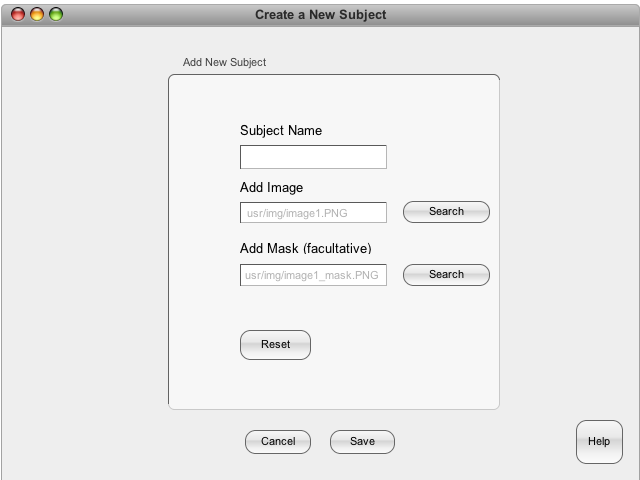
\includegraphics[width=0.75\textwidth]{./Content/Immagini/Prototype-v0.1/filesystemdoc_8_2}
	\caption{Mock-up della pagina di creazione di un nuovo Subject}
	\label{new_subject}
\end{figure}
\subsubsection{Creazione di un gruppo di Subject}
In questa pagina sarà possibile creare un nuovo gruppo di subject\glossario{}, inserendo il \textit{nome} del gruppo, specificandone il \textit{tipo} e selezionando dall'elenco i subject esistenti per il tipo selezionato.
\begin{figure}[htp]
	\centering
	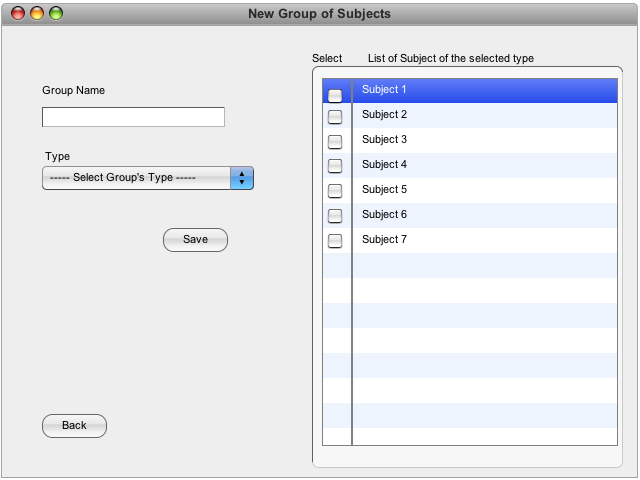
\includegraphics[width=0.75\linewidth]{./Content/Immagini/Prototype-v0.1/filesystemdoc_8_4}
	\caption{Mock-up della pagina di creazione di un gruppo di Subject}
	\label{new_group}
\end{figure}

\subsubsection{Creazione di un Protocol}
In questa pagina sarà possibile creare un nuovo protocol\glossario{}, inserendo il nome del protocol\glossario{}, il tipo, una o più feature\glossario{} e un algoritmo di cluster\glossario{} da applicare per l'analisi.
\begin{figure}[htp]
	\centering
	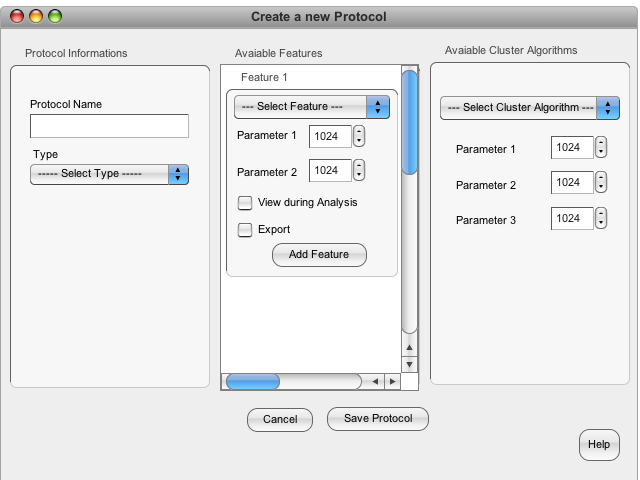
\includegraphics[width=0.75\linewidth]{./Content/Immagini/Prototype-v0.1/filesystemdoc_8_6}
	\caption{Mock-up della pagina di creazione di un Protocol}
	\label{new_protocol}
\end{figure}

\subsubsection{Creazione di un Dataset}
In questa pagina sarà possibile creare un nuovo dataset\glossario{}, inserendo il nome, scegliendo uno dei gruppi di subject\glossario{} esistenti e uno o più protocol\glossario{} da applicare all'analisi.

\begin{figure}[htp]
	\centering
	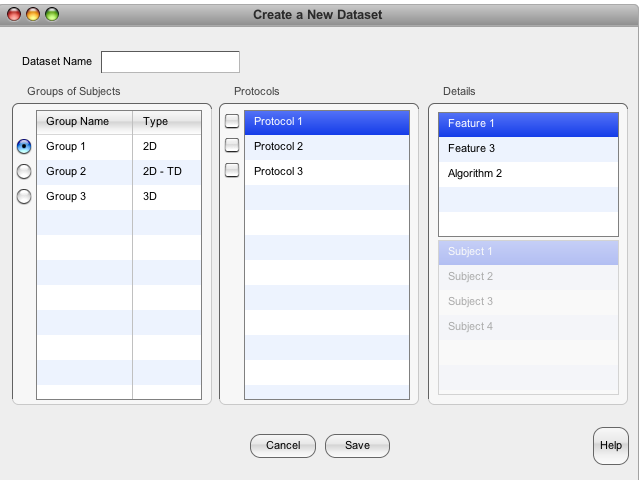
\includegraphics[width=0.75\linewidth,height=7cm]{./Content/Immagini/Prototype-v0.1/filesystemdoc_8_8}
	\caption{Mock-up della pagina di creazione di un Dataset}
	\label{new_dataset}
\end{figure}
\pagebreak
\subsection{Pagine di visualizzazione e modifica}
In queste pagine sarà possibile visualizzare e/o gestire\footnote{La gestione è prevista per tutte le entità tranne che per i subject\glossario{}} le varie entità\footnote{Il termine è da intendersi come sostitutivo di: \textit{subject\glossario{}, gruppi di subject\glossario{}, protocol\glossario{} e dataset\glossario{}} } presenti nel sistema.
A destra verrà visualizzata una lista degli elementi, mentre a sinistra verranno mostrati dei dettagli per ogni elemento selezionato.

\subsubsection{Visualizzazione dei Subject}
In questa pagina verranno visualizzati tutti i subject\glossario{} presenti nel sistema. Per ogni subject\glossario{} verrà visualizzato un pannello contenente i dettagli dell'immagine.
\begin{figure}[htp]
	\centering
	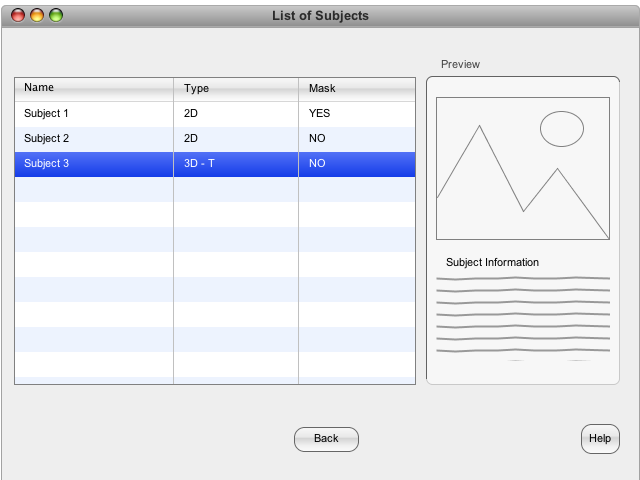
\includegraphics[width=0.75\linewidth,height=6.5cm]{./Content/Immagini/Prototype-v0.1/filesystemdoc_8_3}
	\caption{Mock-up della pagina di visualizzazione dei Subject}
	\label{view_subject}
\end{figure}

\subsubsection{Visualizzazione dei gruppi di Subject}
In questa pagina verranno visualizzati tutti i gruppi di subject\glossario{} presenti nel sistema. Per ogni gruppo selezionato verrà visualizzata la lista dei subject\glossario{} che lo compongono.
\begin{figure}[htp]
	\centering
	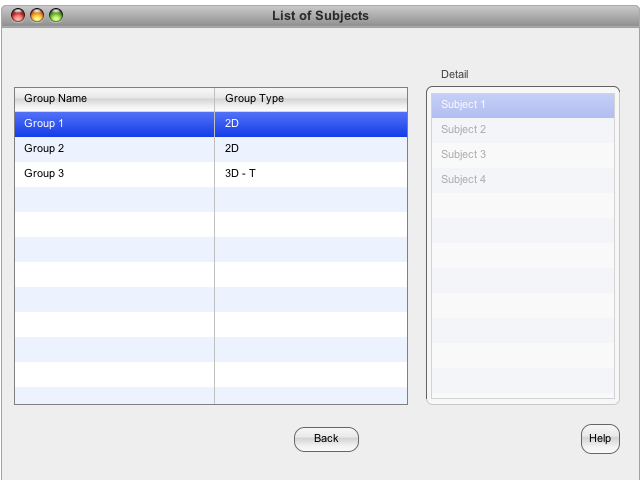
\includegraphics[width=0.75\linewidth,height=6.2cm]{./Content/Immagini/Prototype-v0.1/filesystemdoc_8_5}
	\caption{Mock-up della pagina di visualizzazione dei gruppi di Subject}
	\label{view_group}
\end{figure}

\subsubsection{Visualizzazione dei Protocol}
In questa pagina verranno visualizzati tutti i protocol\glossario{} creati. Per ogni protocol selezionato, verrà visualizzata una lista delle feature\glossario{} che lo compongono.
Sarà inoltre possibile selezionare uno o più protocol\glossario{} per l'eliminazione.
\begin{figure}[htp]
	\centering
	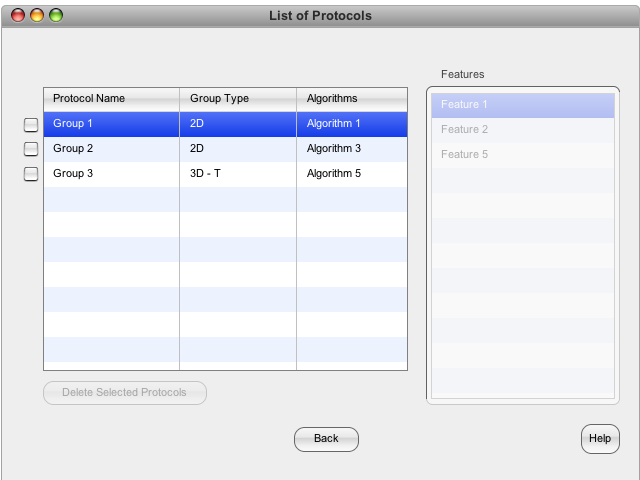
\includegraphics[width=0.8\linewidth,height=7cm]{./Content/Immagini/Prototype-v0.1/filesystemdoc_8_7}
	\caption{Mock-up della pagina di visualizzazione dei gruppi dei Protocol}
	\label{view_protocol}
\end{figure}

\subsubsection{Visualizzazione dei Dataset}
In questa pagina verranno visualizzati i dataset\glossario{} presenti nel sistema. Per ogni dataset\glossario{} verranno visualizzati nel pannello dei dettagli, la lista dei protocol\glossario{}, l'algoritmo di cluster\glossario{}, i subject\glossario{} coinvolti nell'analisi ed eventuali informazioni aggiuntive.
Sarà inoltre possibile selezionare uno o più dataset\glossario{} per l'eliminazione.
\begin{figure}[htp]
	\centering
	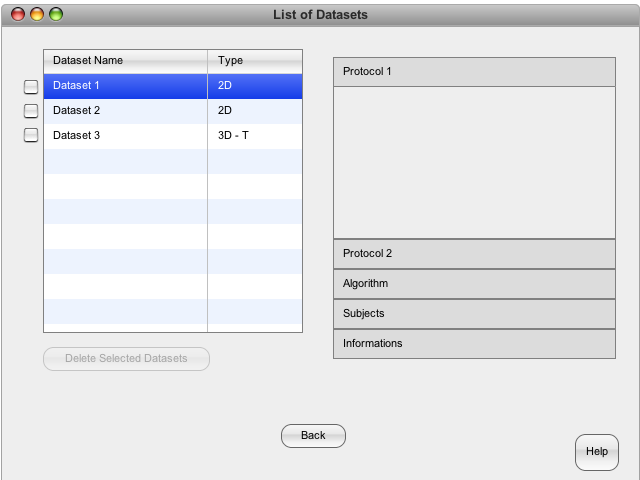
\includegraphics[width=0.8\linewidth,height=7cm]{./Content/Immagini/Prototype-v0.1/filesystemdoc_8_9}
	\caption{Mock-up della pagina di visualizzazione dei Dataset}
	\label{view_dataset}
\end{figure}
\pagebreak
\subsection{Analisi e visualizzazione risultati}
\subsubsection{Avvio analisi}
In questa pagina sarà possibile avviare un'analisi, selezionando un dataset\glossario{} tra quelli presenti nel sistema e specificando eventuali preferenze riguardo alla visualizzazione dei risultati intermedi e/o l'esportazione degli stessi.
\begin{figure}[htp]
	\centering
	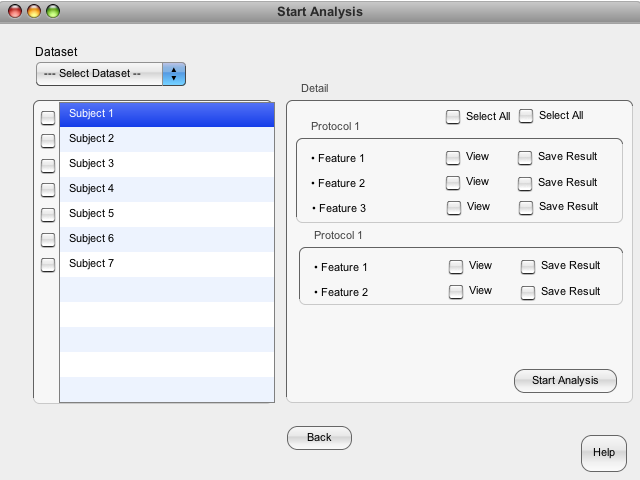
\includegraphics[width=0.8\linewidth,height=7cm]{./Content/Immagini/Prototype-v0.1/filesystemdoc_8_10}
	\caption{Mock-up della pagina di avvio analisi}
	\label{start_analysis}
\end{figure}

\subsubsection{Esecuzione analisi}
Una volta avviata l'analisi, si aprirà una finestra relativa allo stato di avanzamento della stessa. L'utente sarà inoltre in grado di visualizzare eventuali risultati intermedi(se precedentemente selezionati) e di terminare l'analisi in qualsiasi momento.
Una volta che il primo risultato sarà disponibile, l'utente potrà scegliere se continuare a visualizzare i risultati intermedi, attraverso il pulsante \textit{\lq\lq Continue\rq\rq}, viceversa con il pulsante \textit{\lq\lq Continue without showing results\rq\rq}, potrà annullare la visualizzazione.
\begin{figure}[htp]
	\centering
	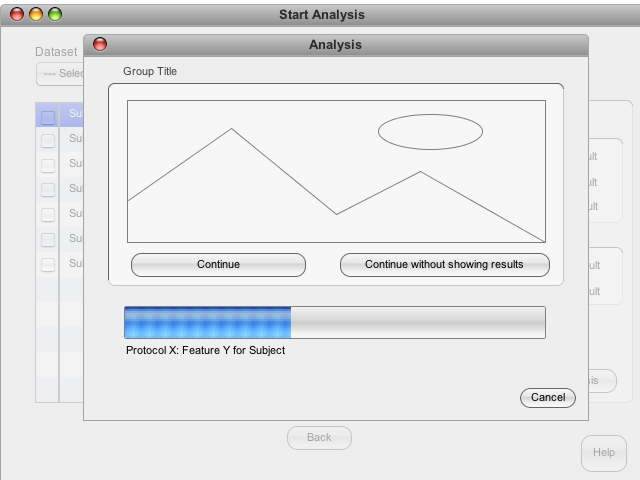
\includegraphics[width=0.8\linewidth,height=7cm]{./Content/Immagini/Prototype-v0.1/filesystemdoc_8_11}
	\caption{Mock-up della finestra di analisi}
	\label{running_analysis}
\end{figure}
\pagebreak

\subsubsection{Visualizzazione risultati}
In questa pagina sarà possibile visualizzare i risultati delle analisi effettuate. Per ogni analisi verranno visualizzati il nome del dataset\glossario{} coinvolto, lo stato dell'analisi (completata o non completata) e la data in cui è stata effettuata. 
Sarà inoltre possibile esportare direttamente tutti i risultati dell'analisi, attraverso il pulsante \textit{\lq\lq Export\rq\rq} o visualizzare una pagina di dettaglio dei risultati, attraverso il link \textit{\lq\lq View Results\rq\rq}.
I risultati potranno essere filtrati per nome, data e stato.
\begin{figure}[htp]
	\centering
	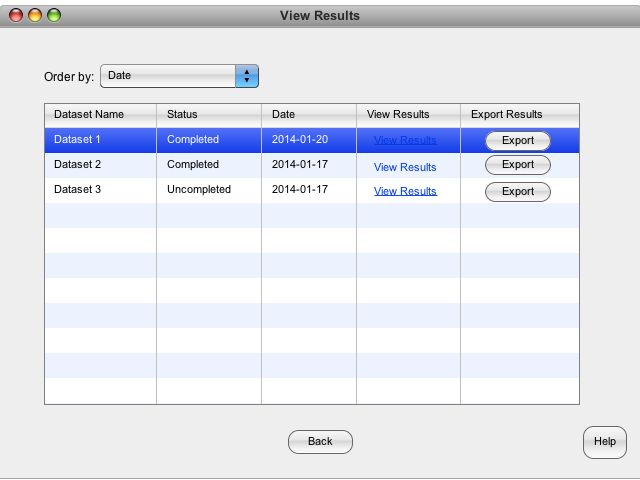
\includegraphics[width=0.8\linewidth,height=7cm]{./Content/Immagini/Prototype-v0.1/filesystemdoc_8_12}
	\caption{Mock-up della finestra dei risultati}
	\label{list_results}
\end{figure}

\subsubsection{Visualizzazione dettaglio risultati}
In questa pagina sarà possibile visualizzare in dettaglio i risultati di un'analisi, filtrati per protocol\glossario{} (fig. \ref{detail_results-protocol}) o per subject\glossario{} (fig.\ref{detail_results-subject}). Sarà possibile quindi, visualizzare un'anteprima delle immagini prima dell'esportazione.
\begin{figure}[htp]
	\centering
	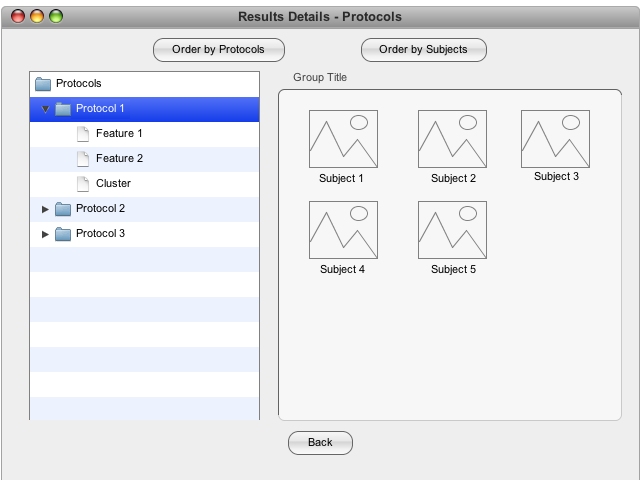
\includegraphics[width=0.80\linewidth,height=7cm]{./Content/Immagini/Prototype-v0.1/filesystemdoc_8_13}
	\caption{Mock-up della finestra di dettaglio dei risultati per Protocol}
	\label{detail_results-protocol}
\end{figure}
\pagebreak
\begin{figure}[!h]
	\centering
	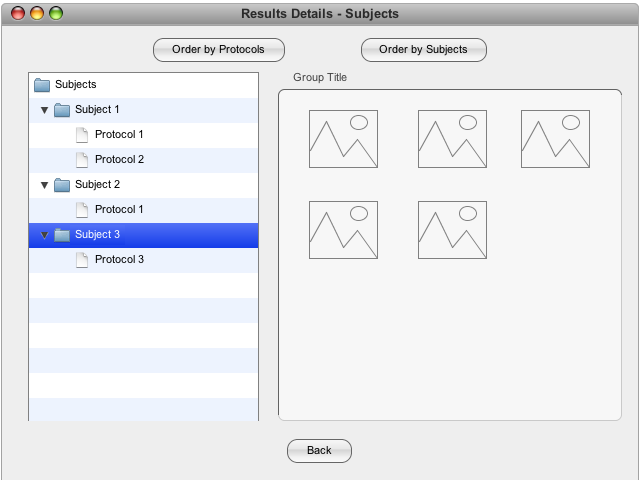
\includegraphics[width=0.8\linewidth,height=7cm]{./Content/Immagini/Prototype-v0.1/filesystemdoc_8_14}
	\caption{Mock-up della finestra di dettaglio dei risultati per Subject}
	\label{detail_results-subject}
\end{figure}